\iffalse
This file is protected by Copyright. Please refer to the COPYRIGHT file
distributed with this source distribution.

This file is part of OpenCPI <http://www.opencpi.org>

OpenCPI is free software: you can redistribute it and/or modify it under the
terms of the GNU Lesser General Public License as published by the Free Software
Foundation, either version 3 of the License, or (at your option) any later
version.

OpenCPI is distributed in the hope that it will be useful, but WITHOUT ANY
WARRANTY; without even the implied warranty of MERCHANTABILITY or FITNESS FOR A
PARTICULAR PURPOSE. See the GNU Lesser General Public License for more details.

You should have received a copy of the GNU Lesser General Public License along
with this program. If not, see <http://www.gnu.org/licenses/>.
\fi

%----------------------------------------------------------------------------------------
% Update the docTitle and docVersion per document
%----------------------------------------------------------------------------------------
\def\docTitle{ZedBoard Getting Started Guide}
\def\docVersion{1.3}
%----------------------------------------------------------------------------------------
\documentclass{article}
\iffalse
This file is protected by Copyright. Please refer to the COPYRIGHT file
distributed with this source distribution.

This file is part of OpenCPI <http://www.opencpi.org>

OpenCPI is free software: you can redistribute it and/or modify it under the
terms of the GNU Lesser General Public License as published by the Free Software
Foundation, either version 3 of the License, or (at your option) any later
version.

OpenCPI is distributed in the hope that it will be useful, but WITHOUT ANY
WARRANTY; without even the implied warranty of MERCHANTABILITY or FITNESS FOR A
PARTICULAR PURPOSE. See the GNU Lesser General Public License for more details.

You should have received a copy of the GNU Lesser General Public License along
with this program. If not, see <http://www.gnu.org/licenses/>.
\fi
\author{} % Force author to be blank
%----------------------------------------------------------------------------------------
% Paper size, orientation and margins
%----------------------------------------------------------------------------------------
\usepackage{geometry}
\geometry{
        letterpaper, % paper type
        portrait,    % text direction
        left=.75in,  % left margin
        top=.75in,   % top margin
        right=.75in, % right margin
        bottom=.75in % bottom margin
 }
%----------------------------------------------------------------------------------------
% Header/Footer
%----------------------------------------------------------------------------------------
\usepackage{fancyhdr} \pagestyle{fancy} % required for fancy headers
\renewcommand{\headrulewidth}{0.5pt}
\renewcommand{\footrulewidth}{0.5pt}
\rhead{\small{ANGRYVIPER Team}}
% \rfoot{\thepage}
%----------------------------------------------------------------------------------------
% Appendix packages
%----------------------------------------------------------------------------------------
\usepackage[toc,page]{appendix}
%----------------------------------------------------------------------------------------
% Defined Commands & Renamed Commands
%----------------------------------------------------------------------------------------
\renewcommand{\contentsname}{Table of Contents}
\renewcommand{\listfigurename}{List of Figures}
\renewcommand{\listtablename}{List of Tables}
%----------------------------------------------------------------------------------------
% Various packages
%----------------------------------------------------------------------------------------
\usepackage[usenames,dvipsnames]{xcolor} % for color names see https://en.wikibooks.org/wiki/LaTeX/Colors
\usepackage{hyperref}  % for linking urls and lists
\usepackage{graphicx}  % for including pictures by file
\usepackage{listings}  % for coding language styles
\usepackage{rotating}  % for sideways table
\usepackage{pifont}    % for sideways table
\usepackage{pdflscape} % for landscape view
\usepackage{subfig}
\usepackage{xstring}
\uchyph=0 % Never hyphenate acronyms like RCC (I think this overrides ANGRYVIPER above)
\renewcommand\_{\textunderscore\allowbreak} % Allow words to break/newline on underscores
%----------------------------------------------------------------------------------------
% Table packages
%----------------------------------------------------------------------------------------
\usepackage{longtable} % for long possibly multi-page tables
\usepackage{tabularx} % c=center,l=left,r=right,X=fill
% These define tabularx columns "C" and "R" to match "X" but center/right aligned
\newcolumntype{C}{>{\centering\arraybackslash}X}
\newcolumntype{R}{>{\raggedleft\arraybackslash}X}
\usepackage{float}
\floatstyle{plaintop}
\usepackage[tableposition=top]{caption}
\newcolumntype{P}[1]{>{\centering\arraybackslash}p{#1}}
\newcolumntype{M}[1]{>{\centering\arraybackslash}m{#1}}
%----------------------------------------------------------------------------------------
% Block Diagram / FSM Drawings
%----------------------------------------------------------------------------------------
\usepackage{tikz}
\usetikzlibrary{shapes,arrows,fit,positioning}
\usetikzlibrary{automata} % used for the fsm
%----------------------------------------------------------------------------------------
% Colors Used
%----------------------------------------------------------------------------------------
\usepackage{colortbl}
\definecolor{blue}{rgb}{.7,.8,.9}
\definecolor{ceruleanblue}{rgb}{0.16, 0.32, 0.75}
\definecolor{drkgreen}{rgb}{0,0.6,0}
\definecolor{deepmagenta}{rgb}{0.8, 0.0, 0.8}
\definecolor{cyan}{rgb}{0.0,0.6,0.6}
\definecolor{maroon}{rgb}{0.5,0,0}
%----------------------------------------------------------------------------------------
% VHDL Coding Language Style
% modified from: http://latex-community.org/forum/viewtopic.php?f=44&t=22076
%----------------------------------------------------------------------------------------
\lstdefinelanguage{VHDL}
{
        basicstyle=\ttfamily\footnotesize,
        columns=fullflexible,keepspaces,      % https://tex.stackexchange.com/a/46695/87531
        keywordstyle=\color{ceruleanblue},
        commentstyle=\color{drkgreen},
        morekeywords={
    library,use,all,entity,is,port,in,out,end,architecture,of,
    begin,and, signal, when, if, else, process, end,
        },
        morecomment=[l]--
}
%----------------------------------------------------------------------------------------
% XML Coding Language Style
% modified from: http://tex.stackexchange.com/questions/10255/xml-syntax-highlighting
%----------------------------------------------------------------------------------------
\lstdefinelanguage{XML}
{
        basicstyle=\ttfamily\footnotesize,
        columns=fullflexible,keepspaces,
        morestring=[s]{"}{"},
        morecomment=[s]{!--}{--},
        commentstyle=\color{drkgreen},
        moredelim=[s][\color{black}]{>}{<},
        moredelim=[s][\color{cyan}]{\ }{=},
        stringstyle=\color{maroon},
        identifierstyle=\color{ceruleanblue}
}
%----------------------------------------------------------------------------------------
% DIFF Coding Language Style
% modified from http://tex.stackexchange.com/questions/50176/highlighting-a-diff-file
%----------------------------------------------------------------------------------------
\lstdefinelanguage{diff}
{
        basicstyle=\ttfamily\footnotesize,
        columns=fullflexible,keepspaces,
        breaklines=true,                                % wrap text
        morecomment=[f][\color{ceruleanblue}]{@@},      % group identifier
        morecomment=[f][\color{red}]-,                  % deleted lines
        morecomment=[f][\color{drkgreen}]+,             % added lines
        morecomment=[f][\color{deepmagenta}]{---},      % Diff header lines (must appear after +,-)
        morecomment=[f][\color{deepmagenta}]{+++},
}
%----------------------------------------------------------------------------------------
% Python Coding Language Style
% modified from
%----------------------------------------------------------------------------------------
\lstdefinelanguage{python}
{
        basicstyle=\ttfamily\footnotesize,
        columns=fullflexible,keepspaces,
        keywordstyle=\color{ceruleanblue},
        commentstyle=\color{drkgreen},
        stringstyle=\color{orange},
        morekeywords={
    print, if, sys, len, from, import, as, open,close, def, main, for, else, write, read, range,
        },
        comment=[l]{\#}
}
%----------------------------------------------------------------------------------------
% Fontsize Notes in order from smallest to largest
%----------------------------------------------------------------------------------------
%    \tiny
%    \scriptsize
%    \footnotesize
%    \small
%    \normalsize
%    \large
%    \Large
%    \LARGE
%    \huge
%    \Huge

\date{Version \docVersion} % Force date to be blank and override date with version
\title{\docTitle}
\lhead{Zedboard Getting Started Guide}
%----------------------------------------------------------------------------------------
\usepackage[T1]{fontenc} % http://tex.stackexchange.com/a/181119
\usepackage{graphicx}
\graphicspath{ {figures/} }
\begin{document}
\maketitle
%\thispagestyle{fancy}
\newpage

	\begin{center}
	\textit{\textbf{Revision History}}
		\begin{table}[H]
		\label{table:revisions} % Add "[H]" to force placement of table
			\begin{tabularx}{\textwidth}{|c|X|l|}
			\hline
			\rowcolor{blue}
			\textbf{Revision} & \textbf{Description of Change} & \textbf{Date} \\
		    \hline
		    v1.1 & Initial Release & 3/2017 \\
            \hline
            v1.2 & Updated for OpenCPI Release 1.2 & 8/2017 \\
            \hline
            v1.3 & Updated for OpenCPI Release 1.3 & 2/2018 \\
            \hline
			\end{tabularx}
		\end{table}
	\end{center}

\newpage

\tableofcontents

\newpage

\section{References}
	This document assumes a basic understanding of the Linux command line (or ``shell'') environment.  The reference(s) in Table 1 can be used as an overview of OpenCPI and may prove useful.
\def\refskipocpiov{}
\def\refcapbottom{}
\iffalse
This file is protected by Copyright. Please refer to the COPYRIGHT file
distributed with this source distribution.

This file is part of OpenCPI <http://www.opencpi.org>

OpenCPI is free software: you can redistribute it and/or modify it under the
terms of the GNU Lesser General Public License as published by the Free Software
Foundation, either version 3 of the License, or (at your option) any later
version.

OpenCPI is distributed in the hope that it will be useful, but WITHOUT ANY
WARRANTY; without even the implied warranty of MERCHANTABILITY or FITNESS FOR A
PARTICULAR PURPOSE. See the GNU Lesser General Public License for more details.

You should have received a copy of the GNU Lesser General Public License along
with this program. If not, see <http://www.gnu.org/licenses/>.
\fi

% This snippet creates the "References" table labeled "table:references"
% It creates three columns: Name, Publisher, Link and then inserts default documents
%
% To skip these defaults, define macros named
% refskipgs to skip "Getting Started"
% refskipig to skip "Installation Guide"
% refskipac to skip "Acronyms and Definitions"
% refskipocpiov to skip "OpenCPI Overview"
%
% See RPM_Installation_Guide.tex for examples
%
% After the defaults, it optionally inserts the "myreferences" macro that
% you defined elsewhere (you put hlines above all lines)
%
% If you want the \caption on the bottom, define "refcapbottom"
\begin{center}
\renewcommand*\footnoterule{} % Remove separator line from footnote
\renewcommand{\thempfootnote}{\arabic{mpfootnote}} % Use Arabic numbers (or can't reuse)
\begin{minipage}{0.9\textwidth}
  \begin{table}[H]
\ifx\refcapbottom\undefined
  \caption {References}
  \label{table:references}
\fi
  \begin{tabularx}{\textwidth}{|C|C|}
    \hline
    \rowcolor{blue}
    \textbf{Title} & \textbf{Link} \\
\ifx\refskipocpiov\undefined
    \hline
    OpenCPI Overview & \githubio{Overview.pdf} \\
\fi
\ifx\refskipac\undefined
    \hline
    Acronyms and Definitions & \githubio{Acronyms\_and\_Definitions.pdf} \\
\fi
\ifx\refskipgs\undefined
    \hline
    Getting Started & \githubio{Getting\_Started.pdf} \\
\fi
\ifx\refskipig\undefined
    \hline
    Installation Guide & \githubio{RPM\_Installation\_Guide.pdf} \\
\fi
\ifx\myreferences\undefined
\else
    \myreferences
\fi
    \hline
  \end{tabularx}
\ifx\refcapbottom\undefined
\else
  \caption {References}
  \label{table:references}
\fi
  \end{table}
\end{minipage}
\end{center}


\newpage
\section{Overview}
This purpose of this document is to allow the user to install OpenCPI on the ZedBoard Development Board.
\section{Prerequisites}
\begin{flushleft}
This guide assumes that the following RPMs are installed:  \\
\begin{table}[H]

		\label{table:rpms}
			\begin{tabularx}{\textwidth}{|c|X|}
			\hline
			\rowcolor{blue}
			\textbf{RPM Name} & \textbf{Description} \\
			\hline
			All prerequisite RPMs & These packages have OpenCPI-specific patches and are provided as RPMs. This packaging ensures they will not conflict with other installed copies by using a nonstandard installation location of \path{/opt/opencpi/prerequisites}. \\
				\hline
				\small{\code{opencpi-*.x86\_64.rpm}} &
								Base installation RPM includes the runtime portion of the Component Development Kit (CDK), scripts for creating the user's workspace, limited documentation, and a read-only \code{ocpi.core} Project containing framework essential components, workers, platforms, etc. \\
				\hline
				\small{\code{opencpi-devel-*.x86\_64.rpm}} &
				Additional header files and scripts for developing new assets as HDL and/or RCC. \\
				\hline
				\small{\code{opencpi-hw-platform-zed-*.noarch.rpm}} &
				Additional files necessary to build the framework targeting specific hardware platforms. Automatically requires the zed sw-platform package. \\
				\hline
				\small{\code{opencpi-project-assets*.noarch.rpm}} &
				The \texttt{ocpi.assets} Project, which contains the remaining supported OpenCPI resources, e.g. additional Platform Support, Workers, Demo Applications, etc. \\
				\hline
				\small{\code{opencpi-sw-platform-xilinx13\_3-*.noarch.rpm}} &
				Additional files necessary to build the framework targeting the xilinx13\_3 software platform. \\
				\hline
			\end{tabularx}
\end{table}
This guide assumes that the Core and Assets projects have user copies and have been registered. Creating user copies of projects is done by using the new\_project\_source script as described in the Getting Started Guide.  registering projects is done by running the command \code{ocpidev register project} at the top level of the project.   \\ \bigskip

The development board that is expected to be used is Digilent's ZedBoard. OpenCPI has been tested on ZedBoard Rev. C and Rev. D. Each has separate limitations (described in Myriad-RF\_1\_Zipper\_Limitations.pdf). An Ethernet cable will need to be be plugged in to the Ethernet port on the board.  The ZedBoard gets an IP Address by using DHCP.  It is a requirement if operating in network mode (discussed later) that the Ethernet cable is connected to a network that uses DHCP\footnote{Static IP addresses are possible but have not been integrated with the OpenCPI startup procedure at this time.}.  \\ \bigskip

There is a micro-USB serial port on the back of the ZedBoard labeled UART. A Male micro-USB cable will need to be plugged into this port to access the serial connection.
\begin{figure}[ht]
	\centerline{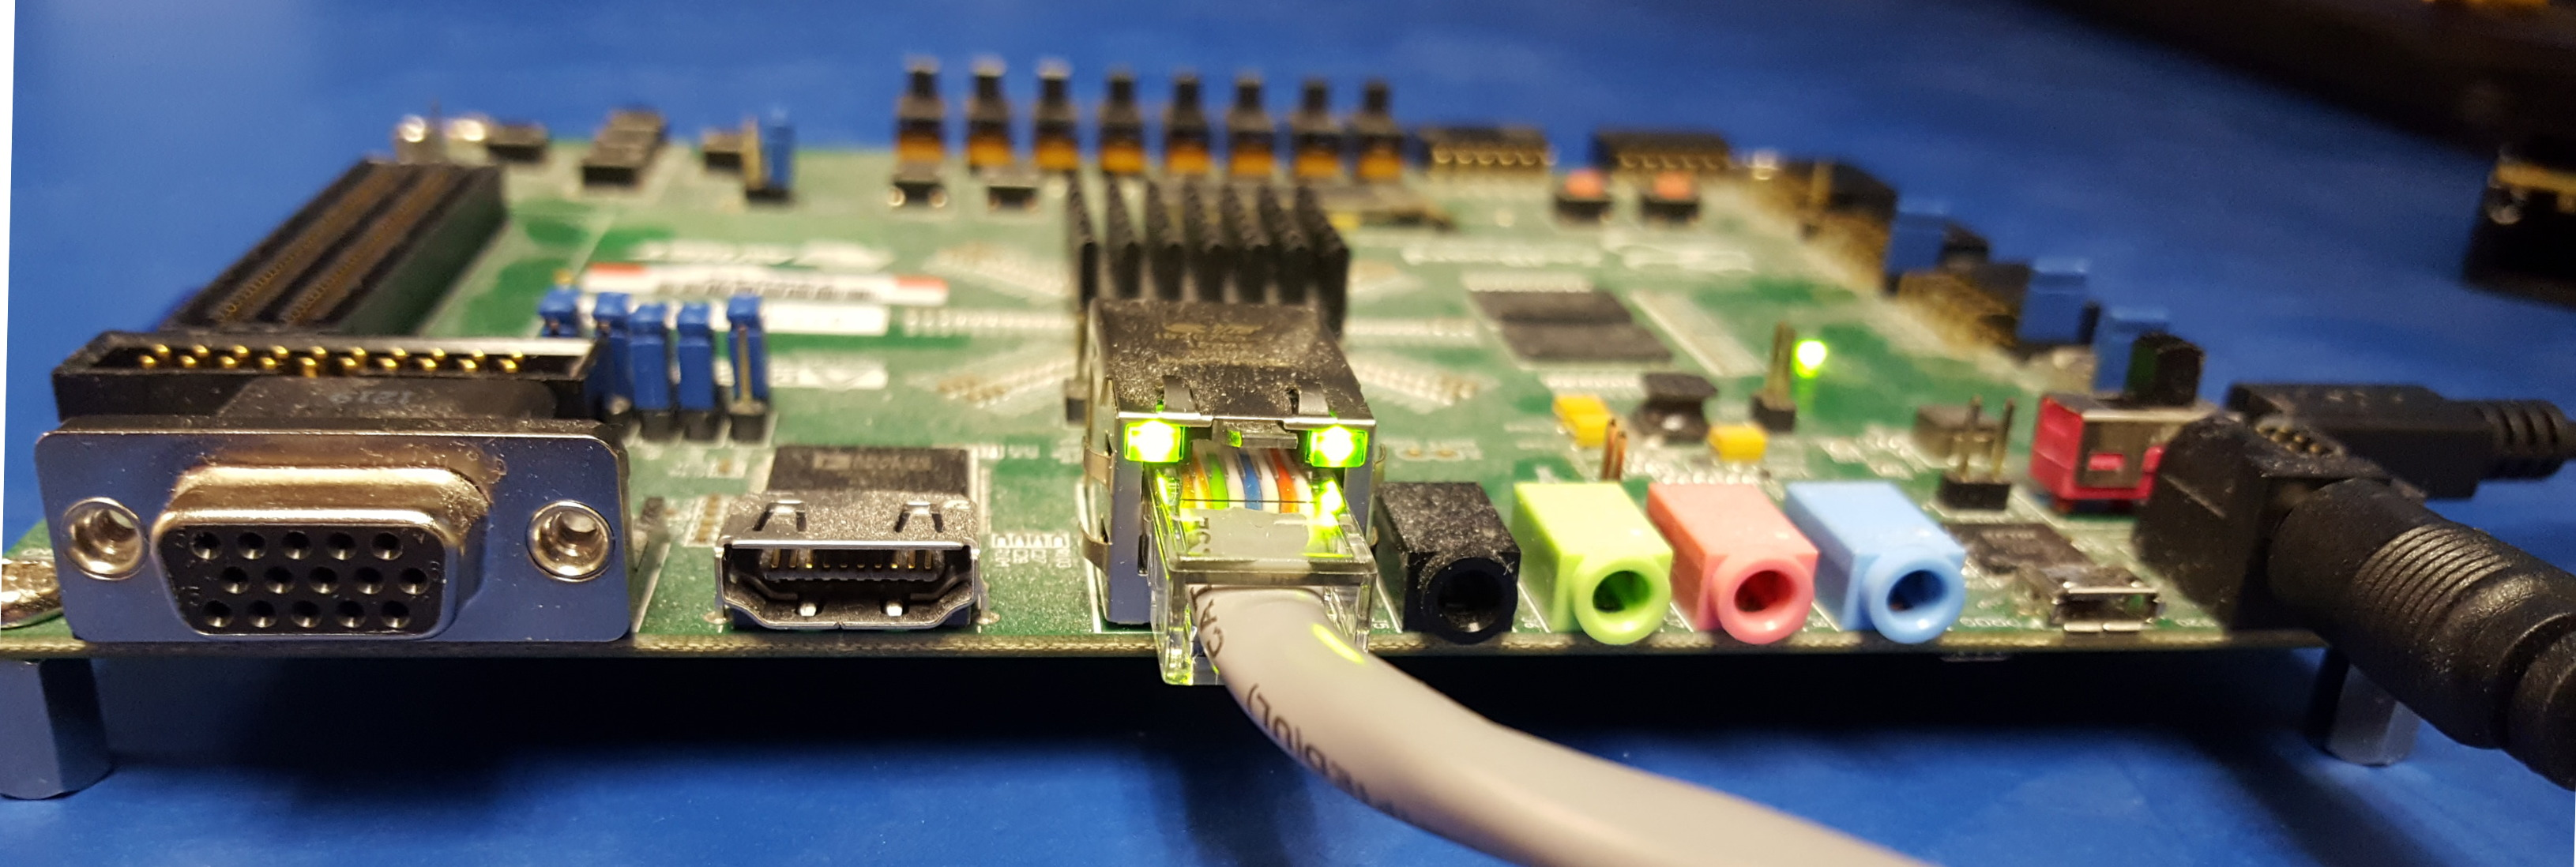
\includegraphics[scale=0.05]{zed_ether}}
	\caption{Connected Ethernet}
	\label{fig:zed_ether}
\end{figure}
\begin{figure}[ht]
	\centerline{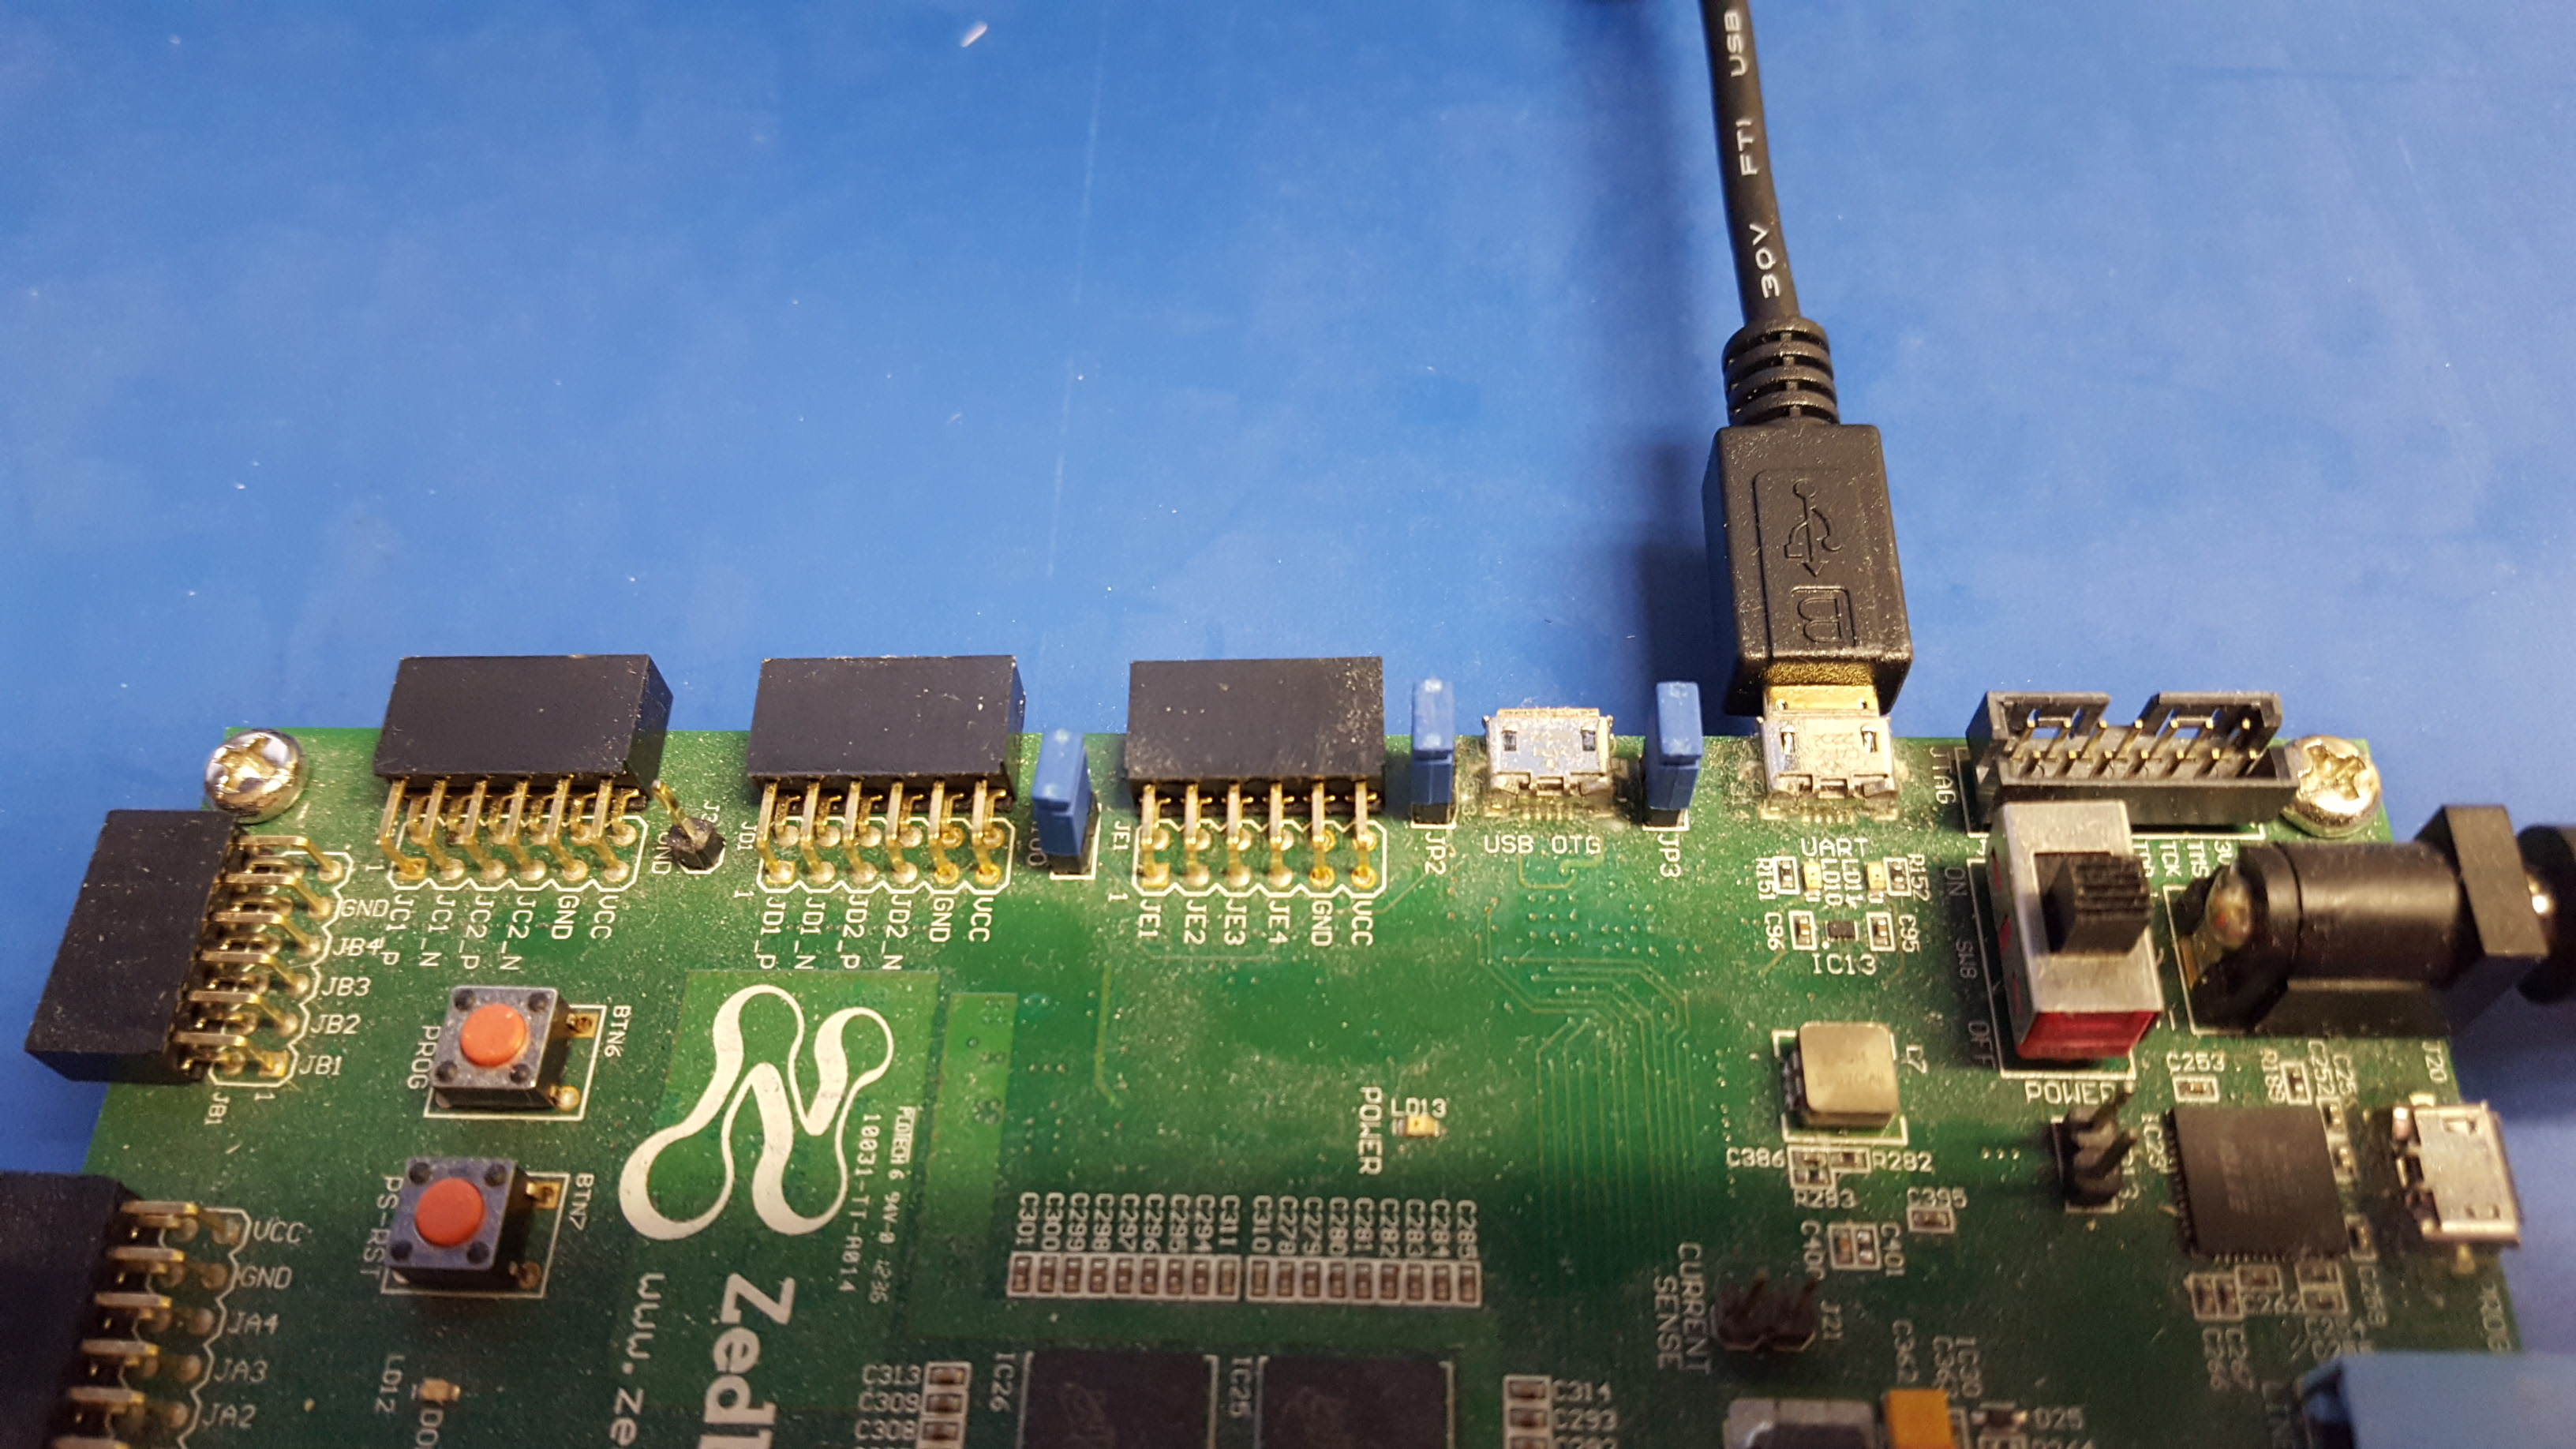
\includegraphics[scale=0.05]{zed_uart}}
	\caption{Connected Serial USB}
	\label{fig:zed_uart}
\end{figure}

\newpage
On one side of the development board, there is a FMC LPC slot. Optionally, this can be used to connect plug-in modules. OpenCPI has been tested with Lime Microsystems' Zipper card with the MyriadRF-1, Analog devices FMCOMMS2, and Analog devices FMCOMMS3 connected to the ZedBoard.\\   \bigskip

Below the FMC LPC slot (underneath the board), is the SD card slot you will be using throughout this guide.
\begin{figure}[ht]
	\centerline{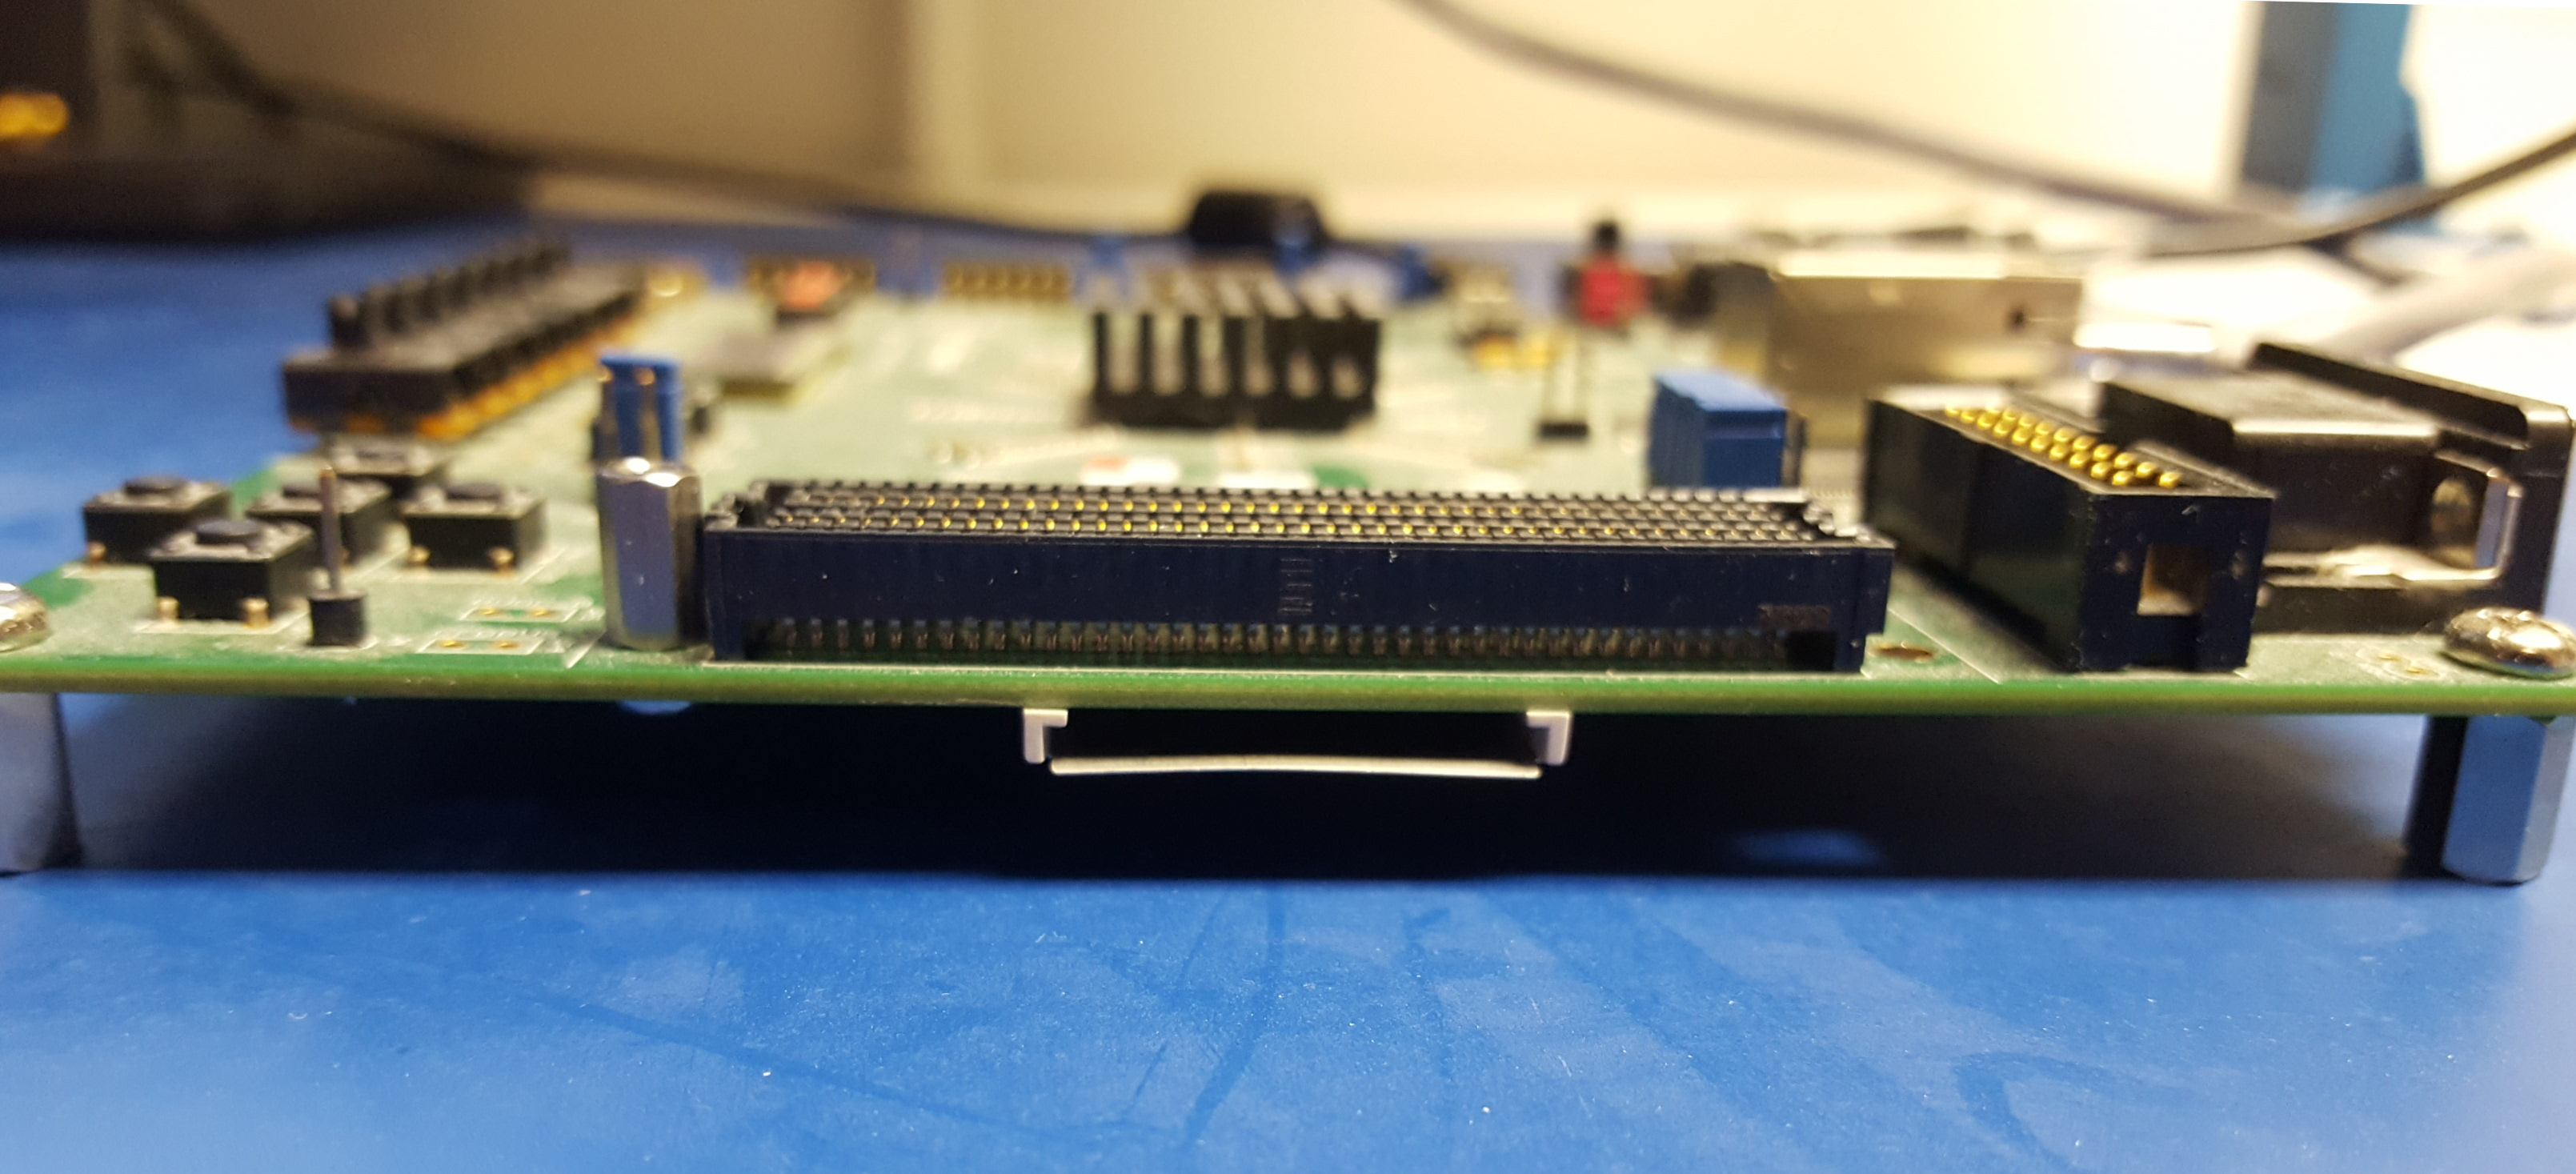
\includegraphics[scale=0.05]{zed_fmc_sd}}
	\caption{ZedBoard FMC Slot and SD card Slot}
	\label{fig:zed_fmc_sd}
\end{figure}
\begin{figure}[ht]
	\centerline{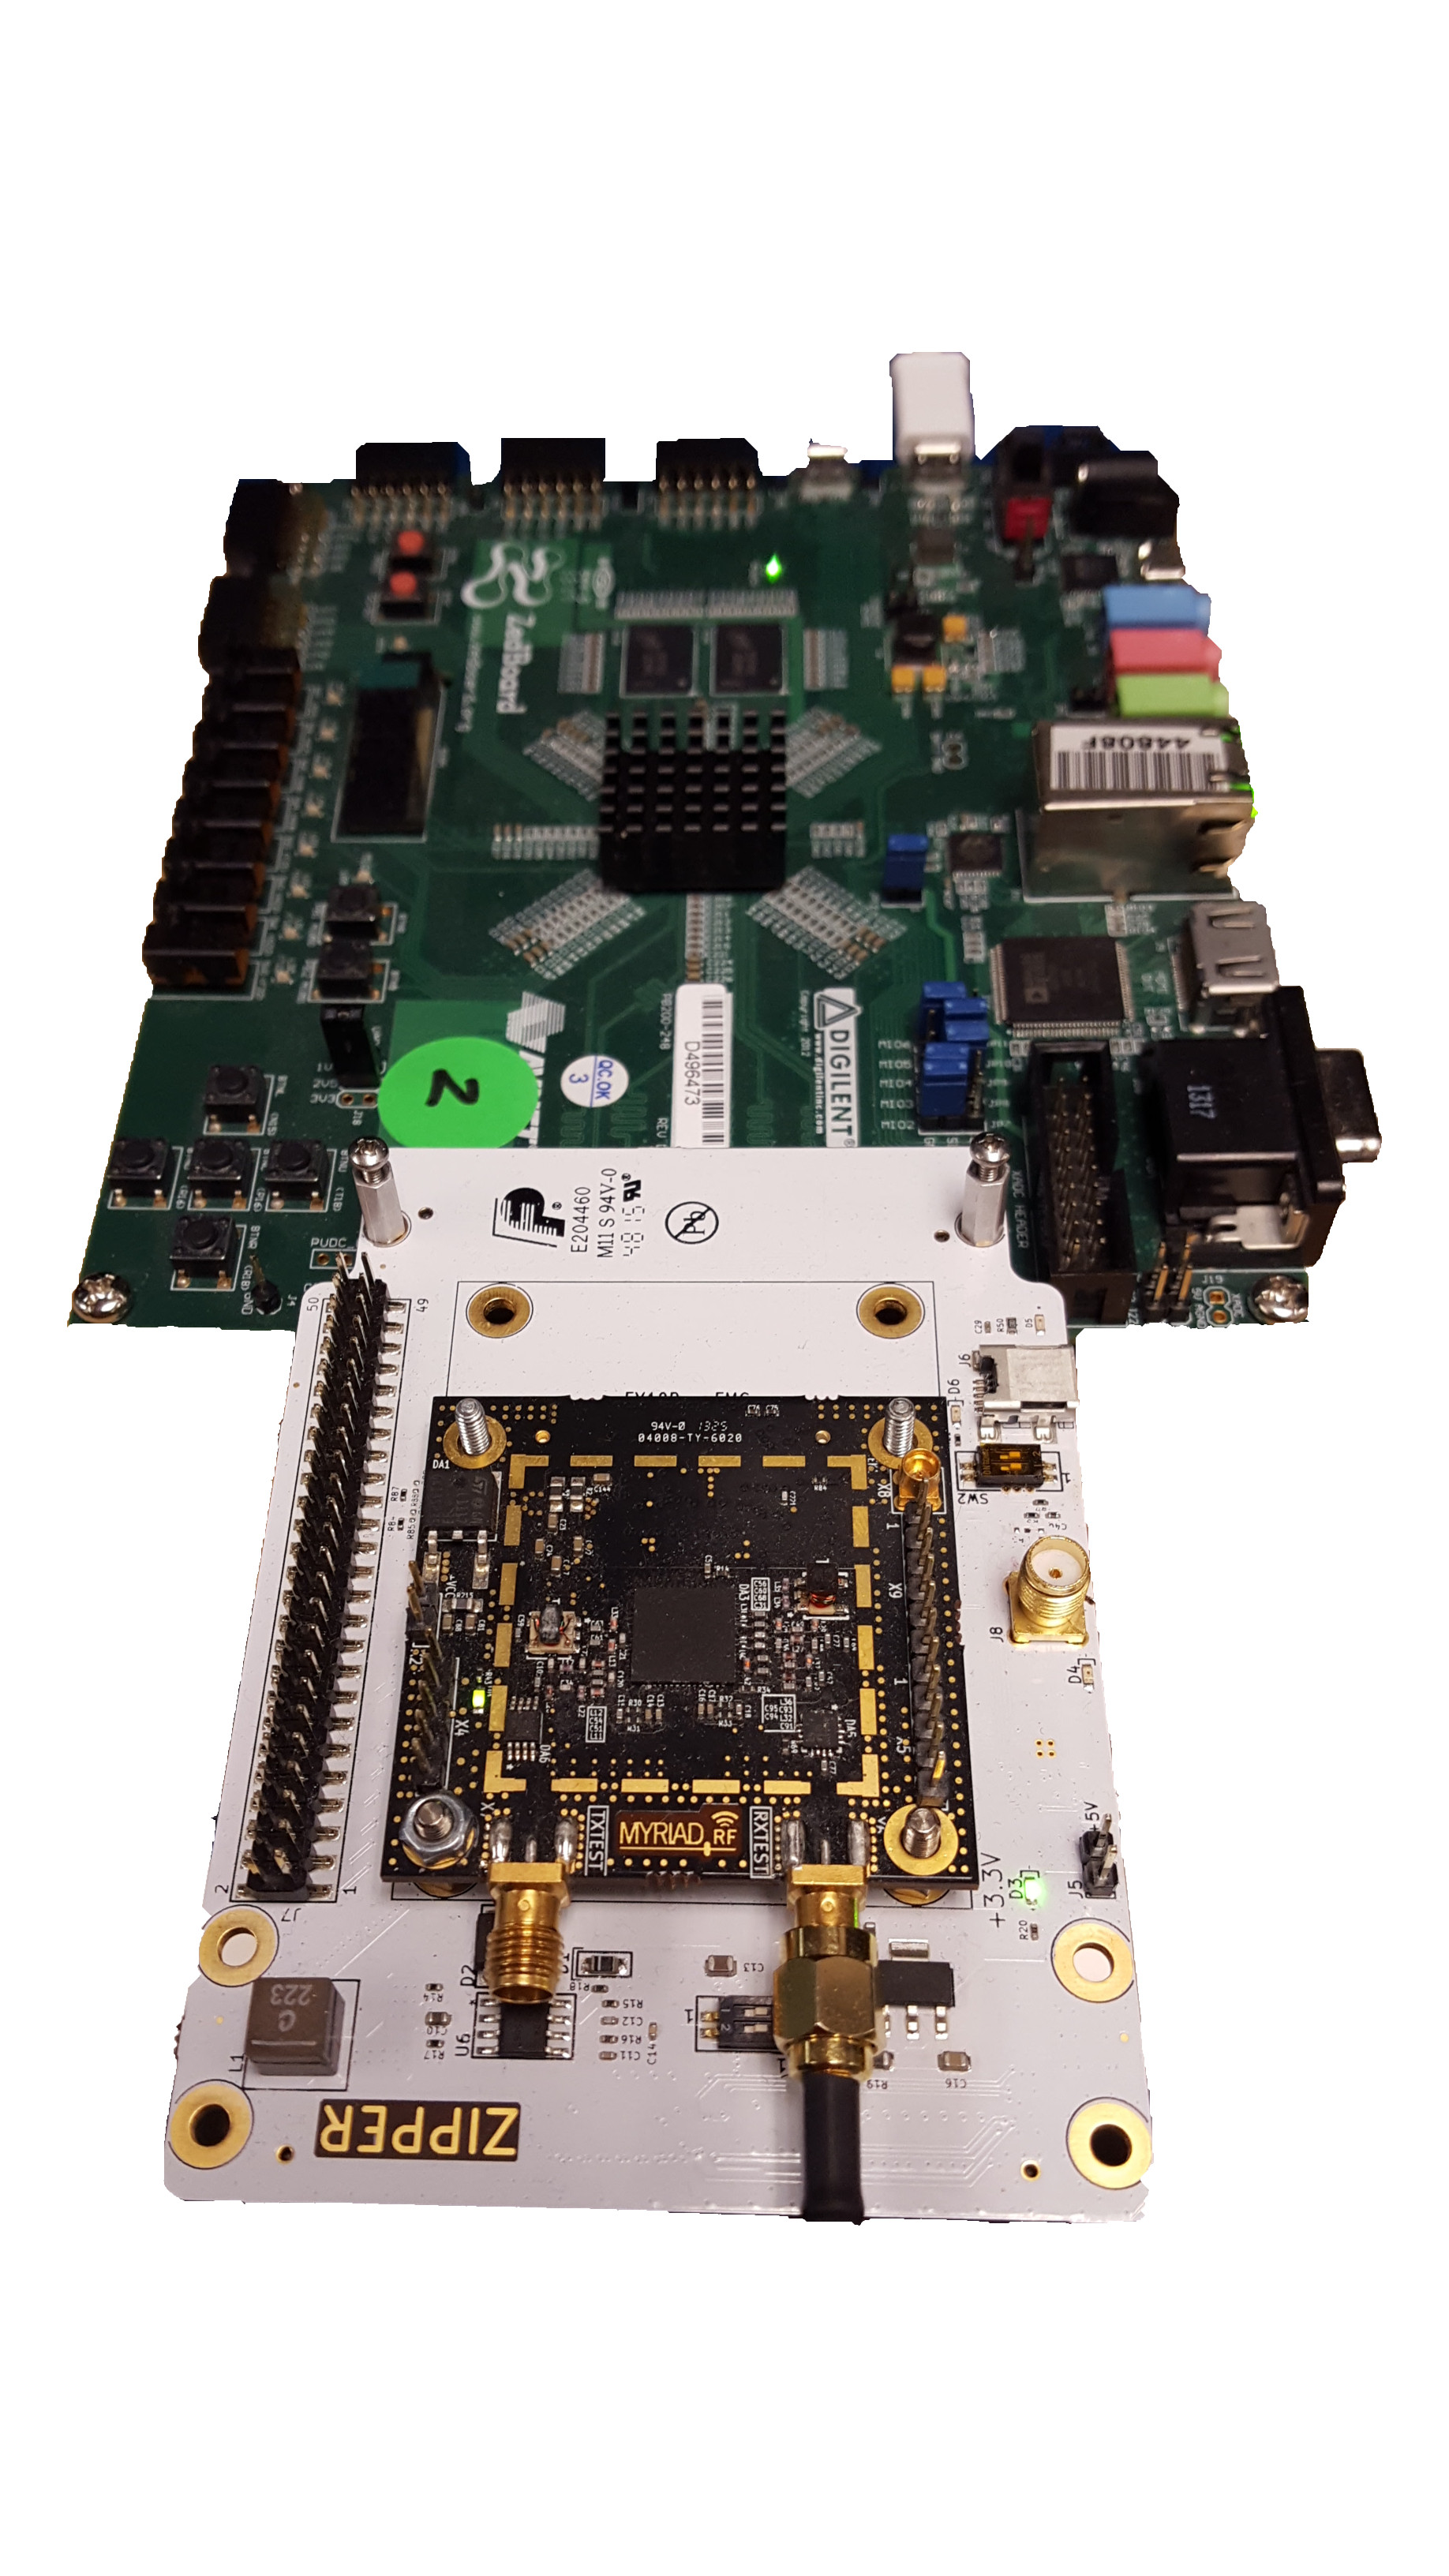
\includegraphics[scale=0.05]{zed_zipper}}
	\caption{ZedBoard With Zipper and MyriadRF-1 Connected to the FMC Slot}
	\label{fig:zed_zipper}
\end{figure}
\end{flushleft}

\section{Script Setup}
There are two modes for running applications on any embedded radio or development board: network mode and standalone mode.  Network mode is when the development system hosts the OpenCPI tree as an NFS server to the ZedBoard as an NFS client.  This configuration provides easy and dynamic access to all of OpenCPI, and presumably any components and applications.  Standalone mode is when all the artifacts are located on the board's local storage (\textit{e.g.} SD card) and no network connection is required.  This is a better \textit{deployment} mode, and is better for situations where a network connection is not possible or practical.  Network mode is generally preferred when it is possible because it makes the development process easier than standalone mode.

\begin{flushleft}
For each mode, there are separate startup scripts that are run on the board. These scripts will need to be modified for each user's specific setup and file structure.  There are starting points for these scripts that are provided by the framework.  For networked mode the script is located at \path{/opt/opencpi/boot_support/zed/OpenCPI-SD-zed/opencpi/default_mynetsetup.sh}.  For standalone mode, the script is located at \path{/opt/opencpi/boot_support/OpenCPI-SD-zed/opencpi/default_mysetup.sh}.  These scripts need to be renamed to \texttt{mynetsetup.sh} and \texttt{mysetup.sh} before they are copied over to the SD card in Section \ref{sec:HW_Setup}. \\ \bigskip

\subsection{Setup for Either Mode}
\texttt{If Linux system time is not required to be accurate, you can skip this step.} \\
\medskip \medskip
\textit{For either usage mode}, the following settings that are passed by \texttt{mynetsetup.sh/mysetup.sh} to the \texttt{zynq\_net\_setup.sh/zynq\_setup.sh} scripts \textit{might} need to be modified:
\end{flushleft}

\begin{itemize}
 \item The system to be used as a time server. Defaulted to ``time.nist.gov''. Change this if you have a local time server that supports RFC-868.
 \item The current timezone description. Defaulted to ``EST5EDT,M3.2.0,M11.1.0''.  Change this if required for the local timezone. See \texttt{man tzset} on the host PC for more information.
 \item If you do not have a time server, or cannot connect to a time server, you will need to manually set the time at start up.  Use the \code{date} command to manually set the Linux system time. See \texttt{man date} on the host PC for more information.
 \end{itemize}

\subsection{Setup for Network Mode}
\begin{flushleft}
\textit{When using Network Mode}, the following modifications are required:
\end{flushleft}

\begin{enumerate}
\item In \texttt{mynetsetup.sh}, find the following lines which are necessary for mounting Assets Project and the Core Project:
\begin{verbatim}
mkdir -p /mnt/ocpi_core
mount -t nfs -o udp,nolock,soft,intr $1:/home/user/ocpiCore /mnt/ocpi_core
mkdir -p /mnt/ocpi_assets
mount -t nfs -o udp,nolock,soft,intr $1:/home/user/ocpiAssets /mnt/ocpi_assets
\end{verbatim}
 \item Edit \texttt{/home/user/ocpiCore} and \texttt{/home/user/ocpiAssets} to reflect the paths to the Core Project and Assets Project on the host. \\
\end{enumerate}

\label{sec:buildNow}
\subsection{Setup for Standalone Mode}
\textit{For Standalone Mode}, all OpenCPI artifacts required to run any applications on the ZedBoard need to be copied onto the SD card.  So, you must build these artifacts earlier when operating in Standalone Mode. Perform the steps in Section \ref{sec:buildverify}  now. The artifacts created will be copied over to the SD card in Section \ref{sec:HW_Setup}. In general, you will want to copy any required \texttt{.so} (RCC workers), \texttt{.bit.gz} (hdl assemblies), and application XMLs or executables onto the SD card.

\subsection{Multiple ZedBoards on the same network}
If you plan to have multiple ZedBoards on one network, you will need to make a change to the zynq startup scripts. This is necessary because by default the ZedBoards will all have the same MAC address. To resolve this, uncomment the following lines in the zynq\_net\_setup.sh and zynq\_setup.sh scripts:
\begin{verbatim}
  # ifconfig eth0 down
  # ifconfig eth0 hw ether 00:0a:35:00:01:23
  # ifconfig eth0 up
  # udhcpc
\end{verbatim}
\section{Hardware and SD Card Setup}
\label{sec:HW_Setup}
\subsection*{Make a backup image of SD card (assumes Linux host)}
This optional section provides the steps for creating an SD card backup image. The following sections assume the SD card is empty.
\begin{itemize}
\item Determine the device file name for the SD card. It will likely be something like \texttt{/dev/sdb} or \texttt{/dev/mmcblk0}. To do this, you can take a look at the end of dmesg: ``\texttt{dmesg | tail -n 15}''.
\item Run the command ``\texttt{dd if=DEVICENAME of=backup.image}'' where DEVICENAME was determined above. This step should take $\sim15$ minutes depending on the card size.
\end{itemize}
\noindent To restore the card back to the original contents, run the command ``\texttt{dd of=DEVICENAME if=backup.image}'' (Do not do this step unless you want the original contents back on the SD card.)
\subsection*{Formatting and populating the SD card}
\begin{itemize}
\item Format the SD card with a single FAT32 partition.
\item Copy the all of the contents of \texttt{/opt/opencpi/boot\_support/OpenCPI-SD-zed/} to this partition.
\end{itemize}
\subsubsection*{Copy the files needed for Standalone Mode to SD card}
\textit{For Standalone Mode}:
\begin{itemize}
\begin{minipage}{\linewidth}
 \item Copy the following files into the \texttt{opencpi/xml} directory on this partition:
 \begin{itemize}
   \item \path{<Assets_Project>/applications/bias.xml}
   \item \path{<Assets_Project>/applications/test.input}
 \end{itemize}
 \item Copy the following files into the \texttt{opencpi/artifacts} directory on this partition:
 \begin{itemize}
   \item \path{<Assets_Project>/hdl/assemblies/testbias/container-testbias_zed_base/target-zynq/testbias_zed_base.bit.gz}
 \end{itemize}
\end{minipage}
\end{itemize}

\newpage
\begin{flushleft}
The SD card file structure should be as follows when these steps have been completed (ellipsis used to denote repetitive files):
\end{flushleft}
\begin{verbatim}
+-- boot.bin
+-- devicetree.dtb
+-- opencpi
|   +-- artifacts
|   |   +-- 001-bias_cc_s.so
       ...
|   |   +-- 020-testzc_s.so
|   |   \-- testbias_zed_base.bit.gz # only in Standalone Mode
|   +-- bin
|   |   +-- ocpibootstrap.sh
|   |   +-- ocpidriver
|   |   +-- ocpihdl
|   |   +-- ocpi_linux_driver
|   |   +-- ocpirun
|   |   +-- ocpiserve
|   |   +-- ocpixml
|   |   \-- ocpizynq
|   +-- default_mynetsetup.sh
|   +-- default_mysetup.sh
|   +-- lib
|   |   \-- linux-x13_3-arm
|   |       +-- libocpi_application_s.so
           ...
|   |       +-- libocpi_util_s.so
|   |       +-- mdev-opencpi.rules
|   |       \-- opencpi-3.10.0-xilinx-dirty-v14.7.ko
|   +-- mynetsetup.sh
|   +-- mysetup.sh
|   +-- system.xml
|   +-- xml
|   |   +-- bias.xml
       ...
|   |   +-- testbias.xml
|   |   +-- test.input # only in Standalone Mode
|   |   \-- time_test.xml
|   +-- zynq_net_setup.sh
|   \-- zynq_setup.sh
+-- uImage
\-- uramdisk.image.gz

\end{verbatim}

\subsection*{Serial setup}
By default, the USB to serial adapter will connect as read-only unless \texttt{udev} rules are added to have the device connect as read write.  Copy the file from the rpm install \path{/opt/opencpi/boot_support/zed/udev.rules/98-zedboard.rules} to \path{/etc/udev/rules.d/}.  This will cause the USB to Serial adapter to connect as \texttt{/dev/zed0} with read and write permissions for all users.  To connect to the serial port, use the command ``\texttt{screen /dev/zed0 115200}''.
\newpage
\subsection*{Boot the ZedBoard from the SD card}
\begin{enumerate}
\item Remove power from the ZedBoard unit.
\item Ensure jumpers are configured correctly
\subitem To boot from the SD card, jumpers JP10, JP9, and JP8 need to be set to 3.3V, 3.3V, and GND respectively as shown below.
\begin{figure}[ht]
	\centerline{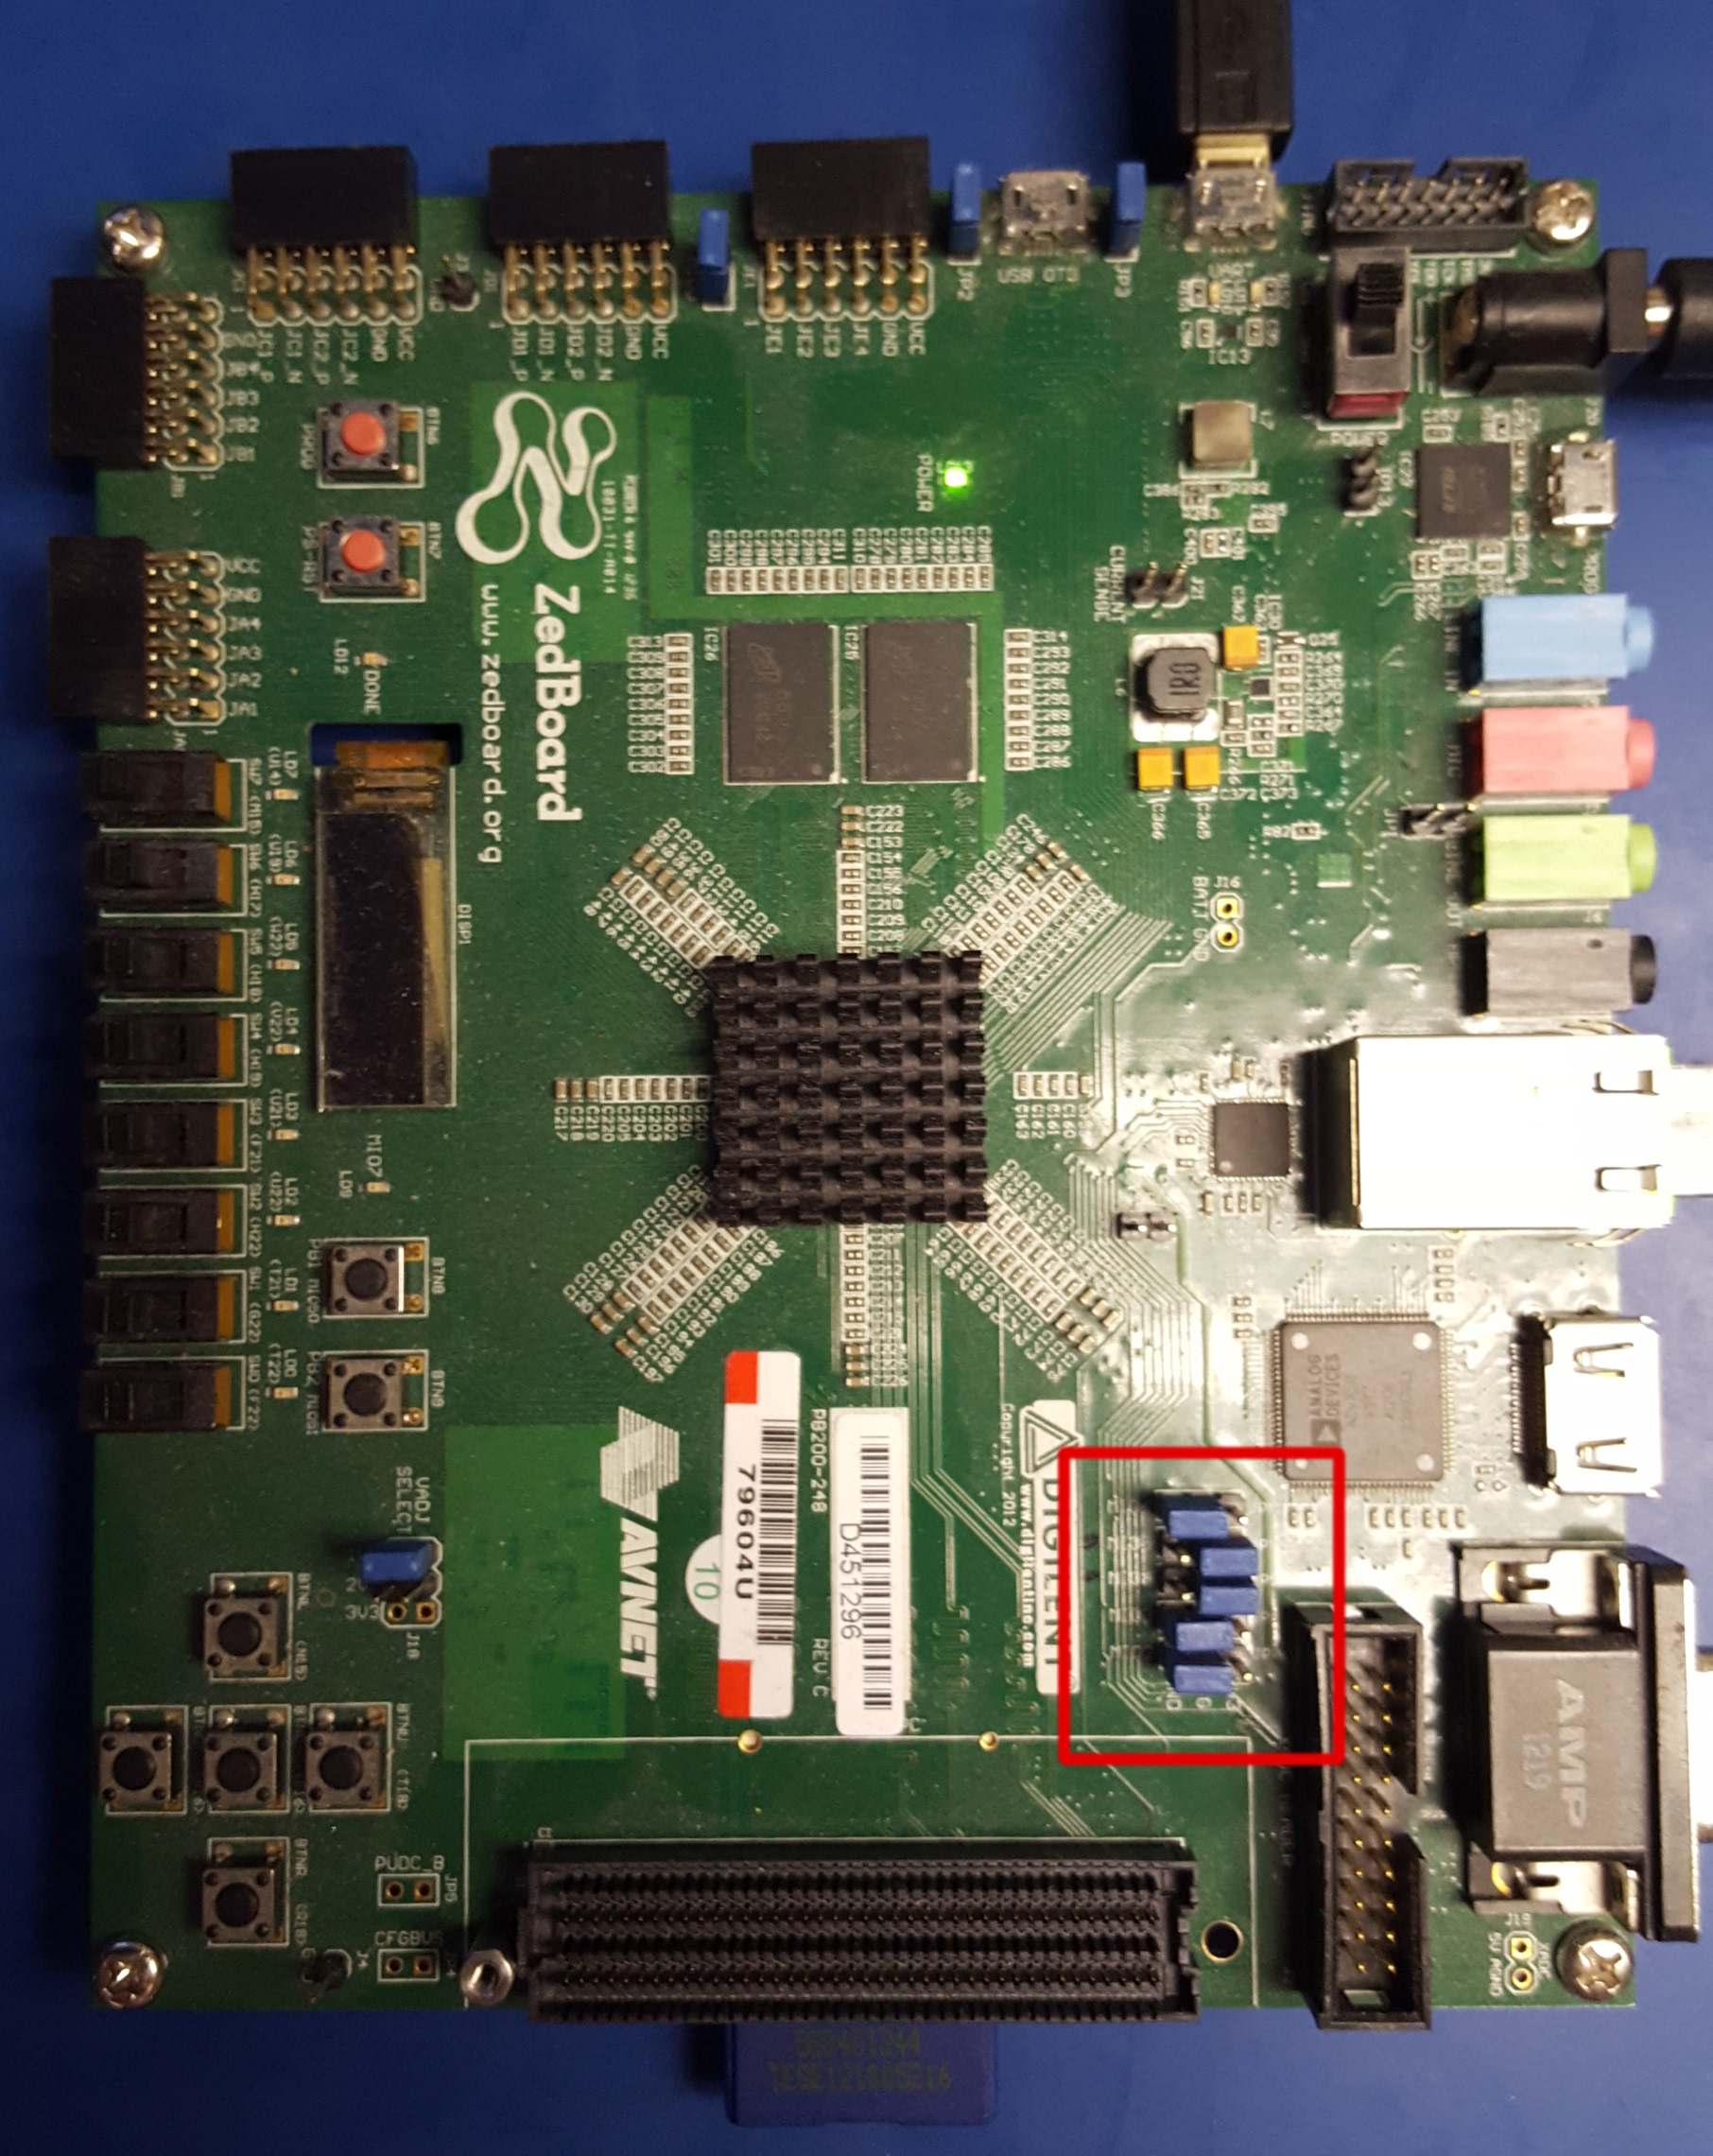
\includegraphics[scale=0.15]{zed_top}}
	\caption{Top View of the ZedBoard with J10, J9, J8 Set}
	\label{fig:zed_top}
\end{figure}
\item Insert the SD card into the SD card slot.
\item Connect a terminal to the micro-USB UART connector of the ZedBoard with a baud rate of 115200.
\begin{itemize}
\item per the previous section, ``\texttt{screen /dev/zed0 115200}'' can be used to connect to the serial port.
\end{itemize}
\item Apply power to the ZedBoard with the terminal still connected.
\end{enumerate}

\section{Software Setup}
% Bring in NFS setup snippet (has subsections)
\iffalse
This file is protected by Copyright. Please refer to the COPYRIGHT file
distributed with this source distribution.

This file is part of OpenCPI <http://www.opencpi.org>

OpenCPI is free software: you can redistribute it and/or modify it under the
terms of the GNU Lesser General Public License as published by the Free Software
Foundation, either version 3 of the License, or (at your option) any later
version.

OpenCPI is distributed in the hope that it will be useful, but WITHOUT ANY
WARRANTY; without even the implied warranty of MERCHANTABILITY or FITNESS FOR A
PARTICULAR PURPOSE. See the GNU Lesser General Public License for more details.

You should have received a copy of the GNU Lesser General Public License along
with this program. If not, see <http://www.gnu.org/licenses/>.
\fi

% This is for inserting into various "Getting Started" Guides
% First, turn off indenting to avoid all the flushleft
\newlength{\savedparindentnfs}%
\setlength{\savedparindentnfs}{\parindent}%
\setlength{\parindent}{0pt} % Don't indent all paragraphs
\providecommand{\forceindent}{\leavevmode{\parindent=1em\indent}}%

\subsection{Network Mounting Mode}
\label{sec:network_mode}
The NFS server needs to be enabled on the host in order to run the SDR in Network Mode.
The following sections are directions on how to do this for both CentOS~6 and CentOS~7 host operating systems.
\subsubsection{CentOS~6}
From the host, install the necessary tools using yum:
\begin{verbatim}
% sudo yum install nfs-utils nfs-utils-lib
% sudo chkconfig nfs on
% sudo service rpcbind start
% sudo service nfs start
\end{verbatim}

From the host, add the following lines to the bottom of \texttt{/etc/exports} and change ``XX.XX.XX.XX/MM'' to a valid netmask for the DHCP range that the SDR will be set to for your network (\textit{e.g.} \texttt{192.168.0.0/16}).
This should be as ``tight'' as possible for security reasons. \textbf{Do \textit{not} share out your top-level directory! This would allow theft of your private ``ssh'' keys, etc!} % AV-5224
\begin{verbatim}
% sudo vi /etc/exports

/opt/opencpi XX.XX.XX.XX/MM(rw,sync,no_root_squash,no_subtree_check)
<host core project location> XX.XX.XX.XX/MM(rw,sync,no_root_squash,no_subtree_check)
<host assets project location> XX.XX.XX.XX/MM(rw,sync,no_root_squash,no_subtree_check)
<host assets_ts project location> XX.XX.XX.XX/MM(rw,sync,no_root_squash,no_subtree_check)

% sudo exportfs -av
\end{verbatim}

From the host, restart the services that have modified for the changes to take effect:
\begin{verbatim}
% sudo service nfs start
\end{verbatim}

\subsubsection{CentOS~7}
From the host, install the necessary tools using yum:\\
~\\
\verb+% sudo yum install nfs-utils+ \footnote{\texttt{nfs-utils-lib} was rolled into \texttt{nfs-utils} starting with CentOS 7.2, if using eariler versions of CentOS 7, \texttt{nfs-utils-lib} will need to be explicitly installed}
~\\

From the host, allow NFS past SELinux\footnote{You can use \texttt{getsebool} to see if these values are already set before attempting to set them. Some security tools may interpret the change attempt as a system attack.}:
\begin{verbatim}
% sudo setsebool -P nfs_export_all_rw 1
% sudo setsebool -P use_nfs_home_dirs 1
\end{verbatim}

From the host, allow NFS past the firewall:
\begin{verbatim}
% sudo firewall-cmd --permanent --zone=public --add-service=nfs
% sudo firewall-cmd --permanent --zone=public --add-port=2049/udp
% sudo firewall-cmd --permanent --zone=public --add-service=mountd
% sudo firewall-cmd --permanent --zone=public --add-service=rpc-bind
% sudo firewall-cmd --reload
\end{verbatim}

Define the export by creating a new file that has the extension ``\texttt{exports}''.
If it does not have that extension, it will be ignored.
Add the following lines to that file and replace ``XX.XX.XX.XX/MM'' with a valid netmask for the DHCP range that the SDR will be set to for your network (\textit{e.g.} \texttt{192.168.0.0/16}).
This should be as ``tight'' as possible for security reasons. \textbf{Do \textit{not} share out your top-level directory! This would allow theft of your private ``ssh'' keys, etc!} % AV-5224

\begin{verbatim}
% sudo vi /etc/exports.d/user_ocpi.exports

/opt/opencpi XX.XX.XX.XX/MM(rw,sync,no_root_squash,crossmnt)
<host core project location> XX.XX.XX.XX/MM(rw,sync,no_root_squash,crossmnt)
<host assets project location> XX.XX.XX.XX/MM(rw,sync,no_root_squash,crossmnt)
<host assets_ts project location> XX.XX.XX.XX/MM(rw,sync,no_root_squash,crossmnt)
\end{verbatim}

If the file system that you are mounting is XFS, then each mount needs to have a unique \texttt{fsid} defined. Instead, use:
\begin{verbatim}
% sudo vi /etc/exports.d/user_ocpi.exports

/opt/opencpi XX.XX.XX.XX/MM(rw,sync,no_root_squash,crossmnt,fsid=33)
<host core project location> XX.XX.XX.XX/MM(rw,sync,no_root_squash,crossmnt,fsid=34)
<host assets project location> XX.XX.XX.XX/MM(rw,sync,no_root_squash,crossmnt,fsid=35)
<host assets_ts project location> XX.XX.XX.XX/MM(rw,sync,no_root_squash,crossmnt,fsid=36)
\end{verbatim}

Restart the services that have modified for the changes to take effect:
\begin{verbatim}
% sudo systemctl enable rpcbind
% sudo systemctl enable nfs-server
% sudo systemctl enable nfs-lock
% sudo systemctl enable nfs-idmap
% sudo systemctl restart rpcbind
% sudo systemctl restart nfs-server
% sudo systemctl restart nfs-lock
% sudo systemctl restart nfs-idmap
\end{verbatim}

* Note: Some of the ``enable'' commands may fail based on your package selection, but should not cause any problems.
\setlength{\parindent}{\savedparindentnfs}%

%

\subsubsection*{Power cycle the ZedBoard}
Make sure the USB cable is plugged into the UART micro-USB port and connected to the network if applicable . The ZedBoard should now boot a valid OpenCPI environment.  The user name and password for the development board are both ``root''.  A successful boot up screen will look as follows:

\begin{figure}[H]
	\centerline{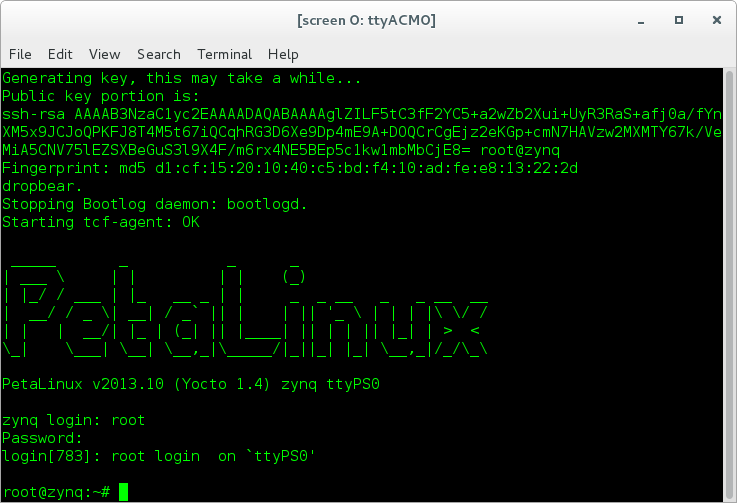
\includegraphics[scale=0.5]{zed_boot}}
	\caption{Successful Boot}
	\label{fig:boot1}
\end{figure}
\subsubsection*{Using the ZedBoard in Network Mode}
\begin{flushleft}
Every time the development board is rebooted, the user is required to run the \texttt{mynetsetup.sh}, which configures the system for OpenCPI with support for network/NFS mode\footnote{This script calls the \texttt{zynq\_net\_setup.sh} script, which is not user-modifiable.}. The user passes the network address of the development system in as the only argument to \texttt{mynetsetup.sh}.
\end{flushleft}
\begin{flushleft}
\newpage
After the development board is booted, the first thing that needs to be done is to source the \texttt{mynetsetup.sh} script with\\
\leavevmode{\parindent=3em\indent}\code{source /mnt/card/mynetsetup.sh XX.XX.XX.XX}\\
and changing XX.XX.XX.XX to the IP address of the NFS host (your development machine, \textit{e.g.} 192.168.1.10). A successful run is shown in Figure~\ref{fig:netsetup}.
\end{flushleft}
\begin{figure}[H]
	\centerline{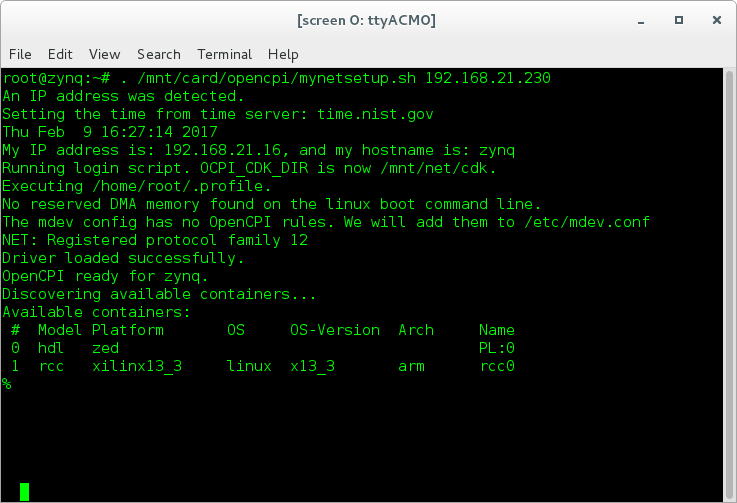
\includegraphics[scale=0.5]{zed_net_setup}}
	\caption{Successful Network Mode Setup}
	\label{fig:netsetup}
\end{figure}
\newpage
\subsection{Standalone Mode}
All artifacts for any applications or tests that need to be located on the SD card must be in the \texttt{opencpi/artifacts} folder.  All of the helper utilities such as \texttt{ocpirun} and \texttt{ocpihdl} are already located on the SD card and do not need to be copied over to the ZedBoard platform.

\subsubsection*{Power cycle the ZedBoard}
The ZedBoard should now boot a valid OpenCPI environment.  The user name and password for the development board are both ``root''.  A successful boot up screen will look as follows:
\begin{figure}[H]
	\centerline{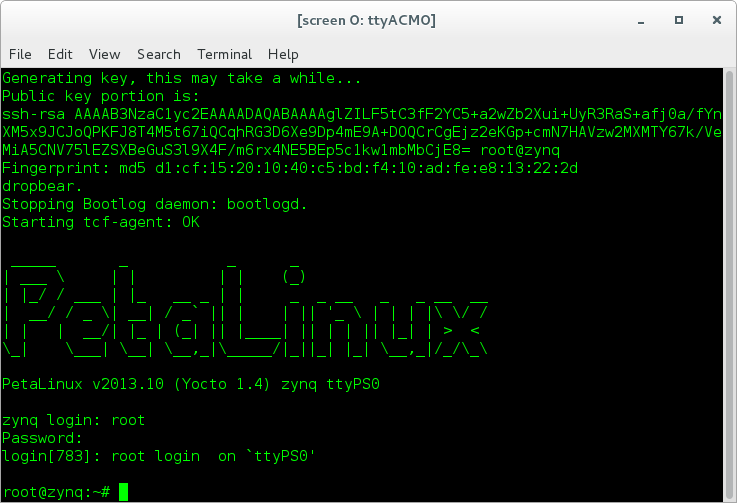
\includegraphics[scale=0.5]{zed_boot}}
	\caption{Successful Boot}
	\label{fig:boot2}
\end{figure}
\newpage
\subsubsection*{Using the ZedBoard in Standalone Mode}
\begin{flushleft}
Every time the development board is rebooted, the user is required to run the \texttt{mysetup.sh}, which configures the system for OpenCPI\footnote{This script calls the \texttt{zynq\_setup.sh} script, which is not user-modifiable.}. Any time that a new version of OpenCPI is released, the SD card will need to be recreated in order to update the artifacts and the executables that are stored on the SD card.
\end{flushleft}
\begin{flushleft}
After the development board is booted, the first thing that needs to be done is to source the \texttt{mysetup.sh} script with\\
\leavevmode{\parindent=3em\indent}\code{source /mnt/card/opencpi/mysetup.sh}\\
A successful run of this will be as follows:
\end{flushleft}


\begin{figure}[H]
	\centerline{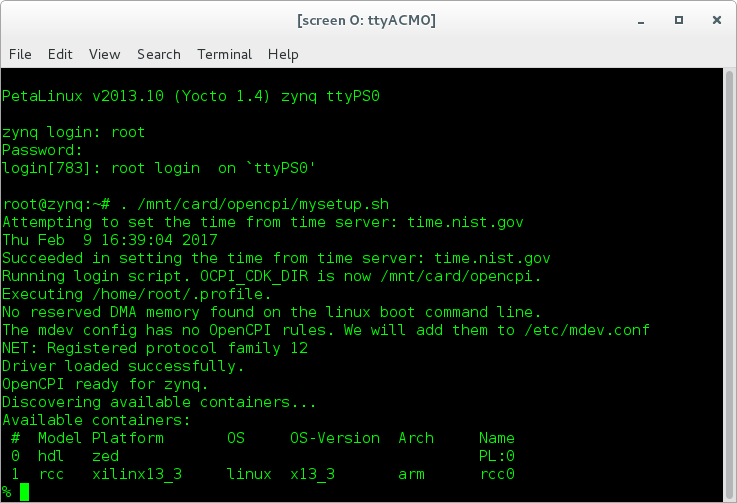
\includegraphics[scale=0.5]{zed_setup}}
	\caption{Successful Standalone Mode Setup}
	\label{fig:standalonesetup}
\end{figure}

\section{Verification}
The installation can be verified by running an application that uses both RCC and HDL workers.  There is an application that uses two RCC and one HDL worker located in \texttt{<Assets Project>/applications/bias.xml}. The two RCC workers are provided pre-built on the SD card or mounted CDK directory.  The HDL worker needs to be built into an assembly before the application can be executed.
\subsection{Building}
\label{sec:buildverify}
If operating in Standalone Mode, these steps should have been performed earlier. (See \ref{sec:buildNow}.)
\\ \\
First the Core project needs to be built for the zed platform.  This is performed at the top level of the Core project running the command \code{ ocpidev build -\--hdl-platforms zed}.  This will take about 45 minutes to complete.
\\ \\
Then the Zed platform needs to be built this is located in the Assets project.  To build this at the top level of the Assets project run the command \code{ocpidev build hdl platform zed}.  This will take about 45 minutes to complete.
\\ \\
There is an existing assembly in the assets project that is the bias worker with its inputs and outputs connected to software.  This assembly needs to be built for ``zed'' platform. It is located in \path{<Assets_Project>/hdl/assemblies/testbias/}.  At the top level of the project run the following command: ``\texttt{ocpidev build hdl assembly testbias -\--hdl-platform zed}''.  This should take about 15 minutes to complete. You can confirm that it succeeded by locating the \texttt{*.bit.gz} file in \path{container-testbias_zed_base/target-zed/}.\\
\newpage
\subsection{Running Network Mode}
The default setup script should already set the \texttt{OCPI\_LIBRARY\_PATH} variable to point to the RCC workers that are required to execute the application, but it needs to be updated to point to the assembly that was built.  After running the \texttt{mynetsetup.sh} script, navigate to  \texttt{/mnt/ocpi\_core/applications}. Update the \texttt{OCPI\_LIBRARY\_PATH} variable using the following command: \\
\texttt{export OCPI\_LIBRARY\_PATH=\$OCPI\_LIBRARY\_PATH:/mnt/ocpi\_assets/hdl/assemblies/}\\

\flushleft In order to run the application, use the following command: ``\texttt{ocpirun -v -t 1 -d -m bias=hdl bias.xml}'' The output should be as follows:
\begin{figure}[H]
	\centerline{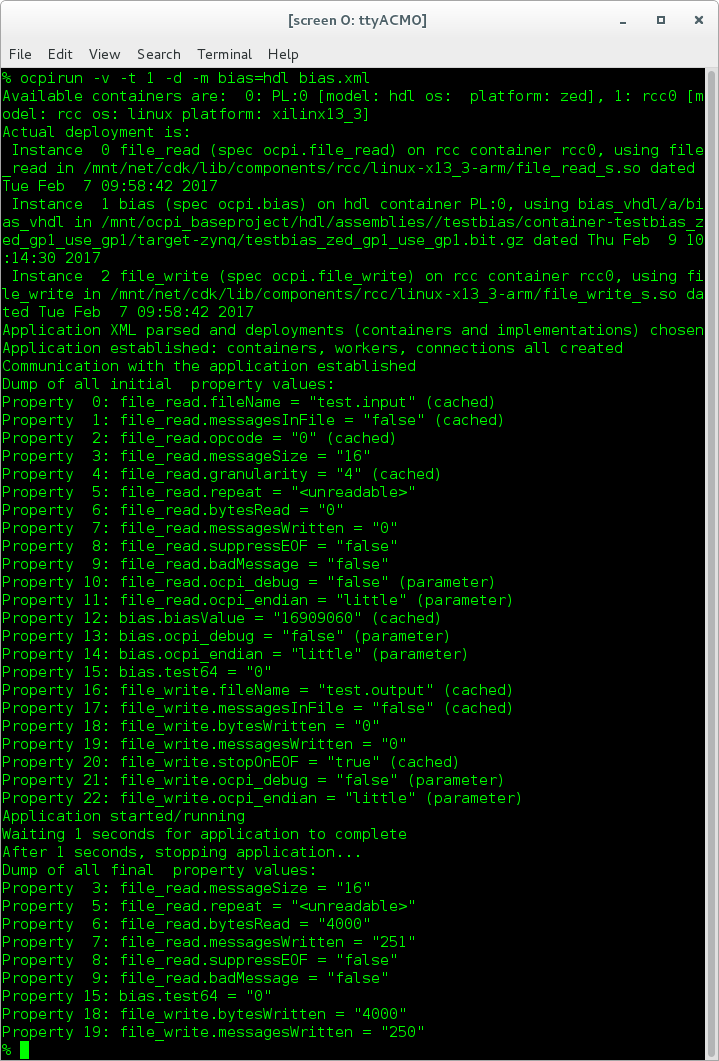
\includegraphics[scale=0.5]{zed_net_bias}}
	\caption{Successful Network Mode Execution}
	\label{fig:netBias}
\end{figure}

\begin{minipage}{\linewidth}
To view the input file, run the following command: ``\code{hexdump test.input | less}'' and the file should look like Figure~\ref{fig:inBias1}: \\ \medskip
\begin{figure}[H]
	\centerline{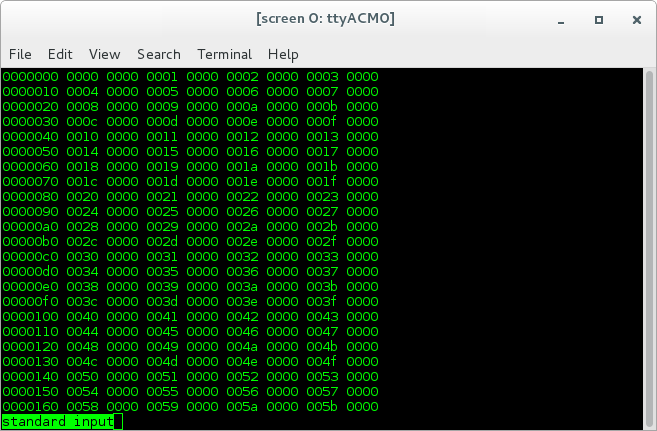
\includegraphics[scale=0.5]{zed_bias_input}}
	\caption{Expected Input}
	\label{fig:inBias1}
\end{figure}
\end{minipage}
~\\
\begin{minipage}{\linewidth}
To view the output file, run the following command: ``\code{hexdump test.output | less}'' and the file should look like Figure~\ref{fig:outBias1}: \\
\begin{figure}[H]
	\centerline{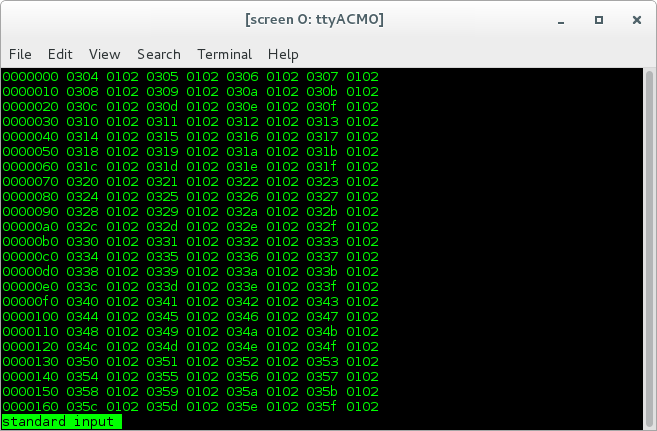
\includegraphics[scale=0.5]{zed_bias_output}}
	\caption{Expected Output}
	\label{fig:outBias1}
\end{figure}
\end{minipage}
~\\
\newpage
\subsection{Running Standalone Mode}
\begin{flushleft}
The default setup script should already set the \texttt{OCPI\_LIBRARY\_PATH} variable to all the required locations for the framework to execute the application.  All three of the artifacts that are located on the SD card are mounted at \texttt{/mnt/card/opencpi/artifacts}.  After running \texttt{mysetup.sh}, navigate to \texttt{/mnt/card/opencpi/xml}.\\
	In order to run the application, use the following command: ``\texttt{ocpirun -v -t 1 -d -m bias=hdl bias.xml}'' The output should be as follows:
\end{flushleft}
\begin{figure}[H]
	\centerline{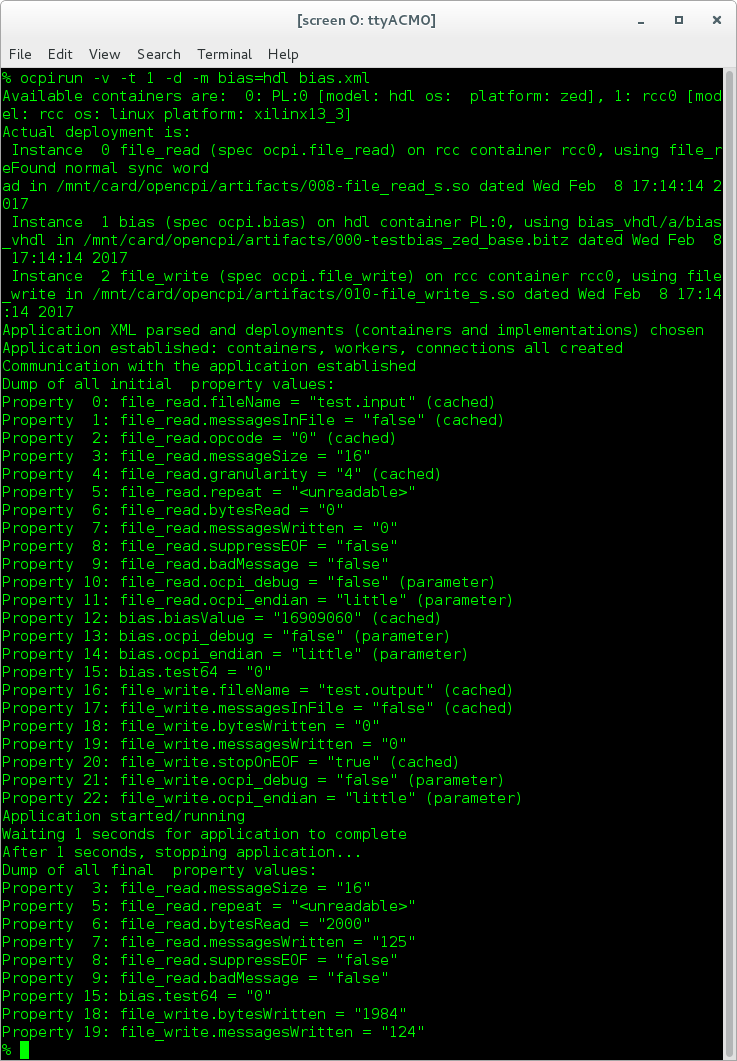
\includegraphics[scale=0.5]{zed_bias}}
	\caption{Successful Standalone Mode Execution}
 \label{fig:standBias}
\end{figure}

\begin{minipage}{\linewidth}
To view the input file, run the following command: ``\code{hexdump test.input | less}'' and the file should look like Figure~\ref{fig:inBias2}: \\ \medskip
\begin{figure}[H]
	\centerline{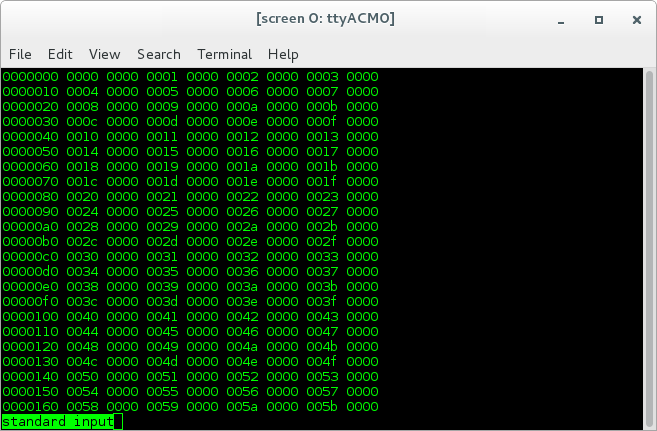
\includegraphics[scale=0.5]{zed_bias_input}}
	\caption{Expected Input}
	\label{fig:inBias2}
\end{figure}
\end{minipage}
~\\
\begin{minipage}{\linewidth}
To view the output file, run the following command: ``\code{hexdump test.output | less}'' and the file should look like Figure~\ref{fig:outBias2}: \\
\begin{figure}[H]
	\centerline{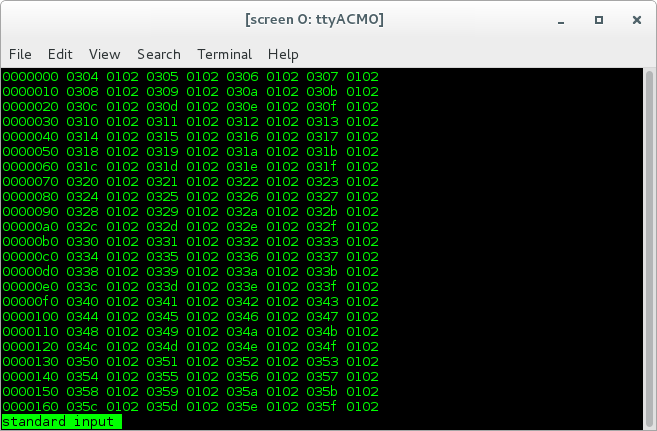
\includegraphics[scale=0.5]{zed_bias_output}}
	\caption{Expected Output}
	\label{fig:outBias2}
\end{figure}
\end{minipage}
~\\

\begin{appendices}
\section{Using ISE instead of Vivado with the ZedBoard}
It is recommended that you use the default toolset (Xilinx Vivado) to build ZedBoard bitstreams with OpenCPI. However, if you wish to use ISE instead, you can use the \code{zed\_ise} platform and \code{zynq\_ise} target. So, instead of ``\code{ocpidev build -\--hdl-platform zed}'', run ``\code{ocpidev build -\--hdl-platform zed\_ise}''. Additionally, you will have to copy the \code{system.xml} file located in \path{<Assets_Project>/hdl/platforms/zed_ise/sd_card/} to the \code{opencpi} directory of the SD card.
% Bring in kernel message snippet
\section{Driver Notes}
\iffalse
This file is protected by Copyright. Please refer to the COPYRIGHT file
distributed with this source distribution.

This file is part of OpenCPI <http://www.opencpi.org>

OpenCPI is free software: you can redistribute it and/or modify it under the
terms of the GNU Lesser General Public License as published by the Free Software
Foundation, either version 3 of the License, or (at your option) any later
version.

OpenCPI is distributed in the hope that it will be useful, but WITHOUT ANY
WARRANTY; without even the implied warranty of MERCHANTABILITY or FITNESS FOR A
PARTICULAR PURPOSE. See the GNU Lesser General Public License for more details.

You should have received a copy of the GNU Lesser General Public License along
with this program. If not, see <http://www.gnu.org/licenses/>.
\fi

% This is for inserting into various "Getting Started" Guides
% First, turn off indenting to avoid all the flushleft
\newlength{\savedparindentdrvr}%
\setlength{\savedparindentdrvr}{\parindent}%
\setlength{\parindent}{0pt} % Don't indent all paragraphs
\providecommand{\forceindent}{\leavevmode{\parindent=1em\indent}}%

When available, the driver will attempt to make use of the CMA region for direct memory access. In use cases where many memory allocations are made, the user may receive the following kernel message:

\lstset{language=bash, backgroundcolor=\color{lightgray}, columns=flexible, breaklines=true, prebreak=\textbackslash, basicstyle=\ttfamily, showstringspaces=false,upquote=true, aboveskip=\baselineskip, belowskip=\baselineskip}
\begin{lstlisting}
alloc_contig_range test_pages_isolated([memory start], [memory end]) failed
\end{lstlisting}

This is a kernel warning, but does not indicate that a memory allocation failure occurred, only that the CMA engine could not allocate memory in the first pass. Its default behavior is to make a second pass and if that succeeded the end user should not see any more error messages. An actual allocation failure will generate unambiguous error messages.

\setlength{\parindent}{\savedparindentdrvr}%

%
\end{appendices}
\end{document}
